\documentclass[fleqn,a4paper,12pt]{article}
\usepackage{standalone}		% Zum Einlesen aus anderen .tex-Files
\usepackage{geometry}		% Zur Bearbeitung des Layouts (Ränder,...)
\geometry{left=30mm, right=40mm, bottom=30mm}
\usepackage[german]{babel}
\usepackage[utf8]{inputenc}
\usepackage{amsmath}		% Mathematische Symbole
\usepackage{amssymb}     	% Nochmehr mathematische Symbole
\usepackage{dsfont}      	% Schriftsatz fuer Zahlenmengensymbole
%\usepackage{verbatim}   	% erweiterte Verbatim-Umgebung
\usepackage{alltt}       	% Quasi-Verbatim-Umgebung
\usepackage{fancyhdr}    	% Eigene Kopfzeilen
\usepackage{graphicx}    	% Zum Einbinden von Grafiken
% Einbinden einer eps-Grafik geht so: includegraphics{path}
\usepackage{wrapfig}
\usepackage{lscape}
\usepackage{rotating}
\usepackage{epstopdf}

% Skalierung der Grafiken
\setlength{\unitlength}{1cm}

\pagestyle{fancy}            % Eigene Kopfzeilen verwenden
\frenchspacing               % Kein Extrafreiraum nach Satzzeichen
\setlength{\parindent}{0pt}  % Neue Absaetze nicht einruecken
%\sloppy                     % Schlampige Absatzformatierung
\fussy                       % Penible Absatzformatierung
\linespread{1.5}             % Zeilenabstand

%andere Definitionen
\newcommand{\R}{{\mathbb R}}
\newcommand{\N}{{\mathbb N}}
\newcommand{\Z}{{\mathbb Z}}
\newcommand{\Q}{{\mathbb Q}}
\newcommand{\C}{{\mathbb C}}
\newcommand{\F}{\mathcal{F}}
\newcommand{\less}{\setminus}
\newcommand{\inv}{{}^{-1}}
\newcommand{\Land}{\bigwedge}
\newcommand{\Lor}{\bigvee}

\begin{document}
	"Ubungsaufgabe 7: \newline
	Aus der Dichtefunktion $p(x) = \lambda e^{-\lambda x}$, $x \geq 0$ ergibt sich die Verteilungsfunktion: \[F(x) = \int p(x) dx = -e^{-\lambda x} + C\]
	Für kontinuierliche Zufallsgrößen ergibt sich der gesuchte \textit{Median} $x_{med}$ folgendermaßen:
	\begin{align*}
	\int_{-\infty}^{x_{med}} p(x) dx &= \frac{1}{2} \\
	\Leftrightarrow \quad \int_0^{x_{med}} p(x) dx &= \frac{1}{2} \quad \text{Da }  p(x) = 0 \text{ für } x < 0 \\
	\Leftrightarrow \left[ -e^{-\lambda x} + C \right]_{0}^{x_{med}} &= \frac{1}{2} \\
	\text{Wähle } \lambda = \frac{1}{2} \\
	\Rightarrow \quad -e^{-\frac{1}{2}x_{med}} + 1 &= \frac{1}{2} \\
	\Rightarrow x_{med} = -2 \cdot \ln \frac{1}{2}
	\end{align*}
	Der Erwartungswert ergibt sich aus \[E(X) = \int_{-\infty}^{+\infty} x \cdot  p(x) dx\] \\
	Lösen des Integrals ergibt dann $E(X) = 2$. \\
	Die Varianz ergibt sich aus \[\textit{Var}(X) = \int_{-\infty}^{+\infty} ( x - E(X) )^2 \cdot p(x) dx\]
	Lösen des Integrals ergibt dann $\textit{Var}(X) = 4$.
	\begin{figure}
		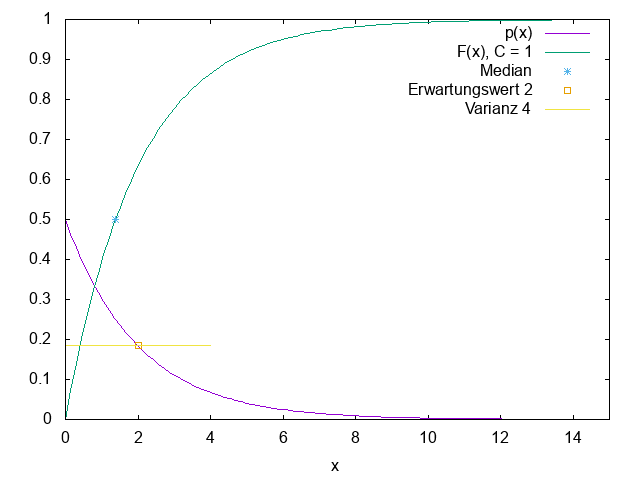
\includegraphics[width=1.0\textwidth]{A07_CDF.png}
		\caption{(7) Darstellung der gegebenen Dichtefunktion und einiger Kenngrößen}
	\end{figure}
\end{document}